\documentclass[aspectratio=169,11pt]{beamer}

\usepackage{amsmath,amssymb}
\usepackage{booktabs}
\usepackage{array}
\usepackage{tikz}
\usepackage{pgfplots}
\pgfplotsset{compat=1.18}
\usetikzlibrary{arrows.meta,positioning,calc}

% ---- Palette ----
\definecolor{navy}{HTML}{1B2A4A}
\definecolor{bred}{HTML}{C0392B}
\definecolor{bgrn}{HTML}{1E8449}
\definecolor{pale}{HTML}{EEF2F7}
\definecolor{steel}{HTML}{5D6D7E}
\definecolor{amber}{HTML}{B7770D}

% ---- Theme ----
\usetheme{default}
\setbeamercolor{frametitle}{bg=navy,fg=white}
\setbeamercolor{title}{fg=navy}
\setbeamercolor{subtitle}{fg=steel}
\setbeamercolor{author}{fg=navy}
\setbeamercolor{structure}{fg=navy}
\setbeamercolor{alerted text}{fg=bred}
\setbeamercolor{example text}{fg=bgrn}
\setbeamercolor{itemize item}{fg=navy}
\setbeamercolor{itemize subitem}{fg=steel}
\setbeamercolor{enumerate item}{fg=navy}
\setbeamercolor{block title}{bg=navy,fg=white}
\setbeamercolor{block body}{bg=pale}
\setbeamercolor{block title alerted}{bg=bred,fg=white}
\setbeamercolor{block body alerted}{bg=pale}
\setbeamercolor{block title example}{bg=bgrn,fg=white}
\setbeamercolor{block body example}{bg=pale}

\setbeamerfont{frametitle}{size=\large,series=\bfseries}
\setbeamerfont{title}{size=\LARGE,series=\bfseries}
\setbeamerfont{block title}{size=\small,series=\bfseries}
\setbeamerfont{block body}{size=\small}

\setbeamertemplate{navigation symbols}{}
\setbeamertemplate{frametitle}{%
  \vspace{0.28em}\insertframetitle\par
  \vspace{0.05em}{\color{bred}\hrule height 0.8pt}\vspace{0.05em}%
}
\setbeamertemplate{footline}{%
  \hfill\textcolor{steel}{\scriptsize\insertframenumber\,/\,\inserttotalframenumber\hspace{1.5em}}%
  \vspace{0.35em}%
}
\setbeamertemplate{itemize item}{\small$\blacktriangleright$}
\setbeamertemplate{itemize subitem}{\small$\triangleright$}

\newcommand{\good}[1]{\textcolor{bgrn}{\textbf{#1}}}
\newcommand{\bad}[1]{\textcolor{bred}{\textbf{#1}}}
\newcommand{\hl}[1]{\textcolor{navy}{\textbf{#1}}}

% ---------------------------------------------------------------
\begin{document}

% ==============================================================
%  TITLE
% ==============================================================
\begin{frame}
\vspace{1.8em}
{\usebeamerfont{title}\usebeamercolor[fg]{title}
Learned Rosters Under Pressure\par}
\vspace{0.3em}
{\color{steel}\small Roster Optimization via Graph-Scored Search and Adversarial Evaluation\par}
\vspace{1.1em}
{\small Luke Blommesteyn \quad \& \quad Jaden Majumdar}\\[0.15em]
{\color{steel}\scriptsize Cassis · Draft}
\vspace{1.3em}
{\color{navy}\hrule height 1pt}
\vspace{0.6em}
{\small Can we select national-team rosters as a formal optimization problem —
producing decisions that are \textit{auditable}, \textit{reproducible}, and \textit{explainable}?}
\end{frame}

% ==============================================================
%  MOTIVATION
% ==============================================================
\begin{frame}{The Problem}
\begin{columns}[T]
\column{0.44\textwidth}
\textbf{How rosters are built today}
\begin{itemize}
  \item Coaches \& scouts — judgment-based
  \item Opaque, inconsistent across evaluators
  \item No mechanism to explain or audit a pick
\end{itemize}
\vspace{0.6em}
\textbf{What we want instead}
\begin{itemize}
  \item A score for every candidate roster
  \item Optimized against realistic opponents
  \item Marginal player value: \emph{why} is this player here?
\end{itemize}

\column{0.52\textwidth}
\centering
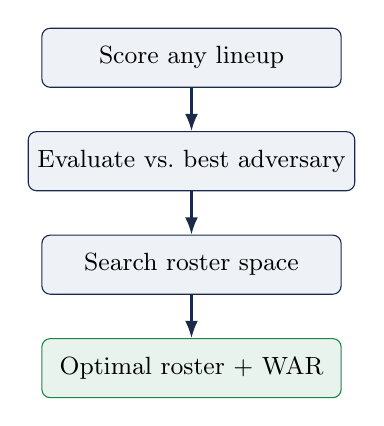
\begin{tikzpicture}[
  node distance=0.55cm,
  pstep/.style={rectangle,draw=navy,fill=pale,rounded corners=3pt,
               minimum width=3.8cm,minimum height=0.75cm,
               align=center,font=\small},
  arr/.style={-{Latex[length=2.2mm]},thick,draw=navy}
]
  \node[pstep] (a) {Score any lineup};
  \node[pstep,below=of a] (b) {Evaluate vs.\ best adversary};
  \node[pstep,below=of b] (c) {Search roster space};
  \node[pstep,below=of c,draw=bgrn,fill=bgrn!10] (d) {Optimal roster + WAR};
  \draw[arr](a)--(b); \draw[arr](b)--(c); \draw[arr](c)--(d);
\end{tikzpicture}
\end{columns}
\end{frame}

% ==============================================================
%  PIPELINE
% ==============================================================
\begin{frame}{How the Pipeline Works}
\centering
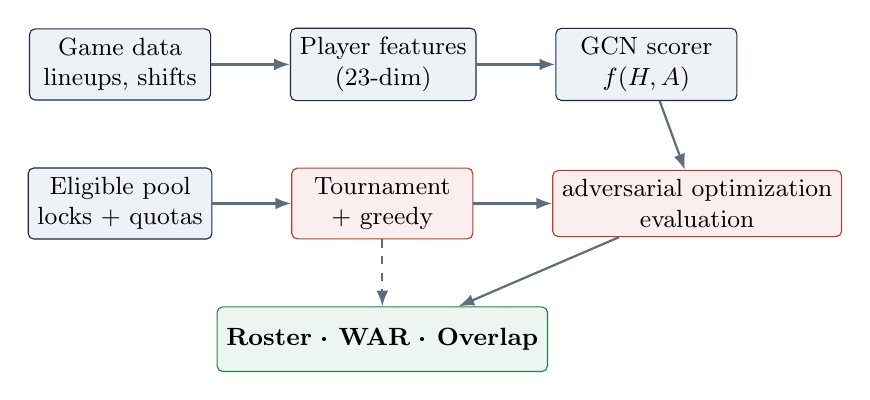
\begin{tikzpicture}[
  box/.style={rectangle,draw=navy,fill=pale,rounded corners=2pt,
              minimum width=2.3cm,minimum height=0.82cm,
              align=center,font=\small},
  ebox/.style={rectangle,draw=bred,fill=bred!8,rounded corners=2pt,
               minimum width=2.3cm,minimum height=0.82cm,
               align=center,font=\small},
  obox/.style={rectangle,draw=bgrn,fill=bgrn!8,rounded corners=2pt,
               minimum width=2.3cm,minimum height=0.82cm,
               align=center,font=\small\bfseries},
  arr/.style={-{Latex[length=2mm]},thick,draw=steel},
  node distance=0.5cm and 1.0cm
]
  \node[box]  (data) {Game data\\lineups, shifts};
  \node[box,right=of data]  (feat) {Player features\\(23-dim)};
  \node[box,right=of feat]  (gcn)  {GCN scorer\\$f(H,A)$};
  \node[box,below=0.85cm of data] (pool) {Eligible pool\\locks + quotas};
  \node[ebox,right=of pool] (srch) {Tournament\\+ greedy};
  \node[ebox,right=of srch] (stck) {adversarial optimization\\evaluation};
  \node[obox,below=0.85cm of srch] (out)  {Roster · WAR · Overlap};
  \draw[arr](data)--(feat); \draw[arr](feat)--(gcn);
  \draw[arr](pool)--(srch); \draw[arr](srch)--(stck);
  \draw[arr](gcn)--(stck);  \draw[arr](stck)--(out);
  \draw[arr,dashed](srch)--(out);
\end{tikzpicture}

\vspace{0.6em}
\begin{columns}[c]
\column{0.32\textwidth}\centering
{\color{navy}\textbf{GCN}} \\[-0.1em]
{\small Learns lineup chemistry from 6,100+ games}
\column{0.32\textwidth}\centering
{\color{bred}\textbf{adversarial optimization}} \\[-0.1em]
{\small Scores against an adversarially optimal opponent}
\column{0.32\textwidth}\centering
{\color{bgrn}\textbf{Search}} \\[-0.1em]
{\small Tournament + greedy narrows $10^{28}$ to one roster}
\end{columns}
\end{frame}

% ==============================================================
%  GCN
% ==============================================================
\begin{frame}[shrink=8]{Scoring Lineups with a Graph Network}
\begin{columns}[T]
\column{0.50\textwidth}
A game is a graph: players are nodes, edges are weighted by \hl{shared on-ice/court time}.

\vspace{0.5em}
\begin{enumerate}
  \item \textbf{Propagate} — 6-layer GCN carries chemistry signals through common teammates, not just direct co-occurrence
  \item \textbf{Aggregate} — DeepSet pools each roster into a lineup vector; order-invariant by design
  \item \textbf{Predict} — antisymmetric head gives $f(H,A) = 1 - f(A,H)$, the win probability
\end{enumerate}

\vspace{0.4em}
Trained on 6,100+ NBA games and 5 NHL seasons.

\column{0.46\textwidth}
\centering
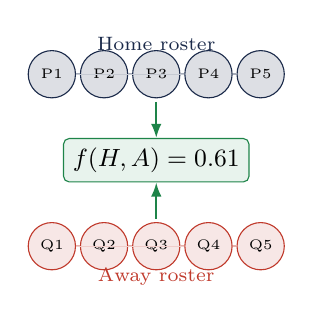
\begin{tikzpicture}[scale=0.78]
  % Home nodes
  \foreach \i/\name in {1/P1,2/P2,3/P3,4/P4,5/P5}{
    \node[circle,draw=navy,fill=navy!15,minimum size=0.6cm,
          font=\tiny,inner sep=1pt]
      (h\i) at ({(\i-3)*0.85}, 1.4) {\name};
  }
  % Away nodes
  \foreach \i/\name in {1/Q1,2/Q2,3/Q3,4/Q4,5/Q5}{
    \node[circle,draw=bred,fill=bred!12,minimum size=0.6cm,
          font=\tiny,inner sep=1pt]
      (a\i) at ({(\i-3)*0.85}, -1.4) {\name};
  }
  % Home edges
  \foreach \i in {1,2,3,4}{
    \pgfmathtruncatemacro{\j}{\i+1}
    \draw[navy!40,line width=0.8pt] (h\i)--(h\j);
  }
  \draw[navy!25,line width=0.5pt] (h1)--(h3); \draw[navy!25,line width=0.5pt] (h2)--(h4);
  % Away edges
  \foreach \i in {1,2,3,4}{
    \pgfmathtruncatemacro{\j}{\i+1}
    \draw[bred!40,line width=0.8pt] (a\i)--(a\j);
  }
  \draw[bred!25,line width=0.5pt] (a1)--(a3); \draw[bred!25,line width=0.5pt] (a2)--(a4);
  % Score output
  \node[rectangle,draw=bgrn,fill=bgrn!10,rounded corners=2pt,
        font=\small\bfseries] (score) at (0,0) {$f(H,A) = 0.61$};
  \draw[-{Latex[length=1.8mm]},bgrn,thick] (0,0.95)--(score);
  \draw[-{Latex[length=1.8mm]},bgrn,thick] (0,-0.95)--(score);
  \node[font=\scriptsize,color=navy] at (0, 1.9) {Home roster};
  \node[font=\scriptsize,color=bred] at (0,-1.9) {Away roster};
\end{tikzpicture}
\end{columns}
\end{frame}

% ==============================================================
%  ADVERSARIAL EVAL — WHAT IS IT
% ==============================================================
\begin{frame}{Adversarial Evaluation — The Core Idea}
\begin{columns}[T]
\column{0.50\textwidth}
A \hl{leader-follower game} played for each candidate roster:

\vspace{0.5em}
\begin{enumerate}
  \item \textbf{We commit} — pick the deployment strategy that maximizes our GCN score
  \item \textbf{Opponent adapts} — observes our deployment and chooses the counter that \emph{minimizes} our score
  \item \textbf{We iterate} — re-optimize against the counter, 100 gradient steps, leader updates 5:1
\end{enumerate}
\vspace{0.4em}
Final score = average over 3 proxy opponents.

\column{0.46\textwidth}
\centering
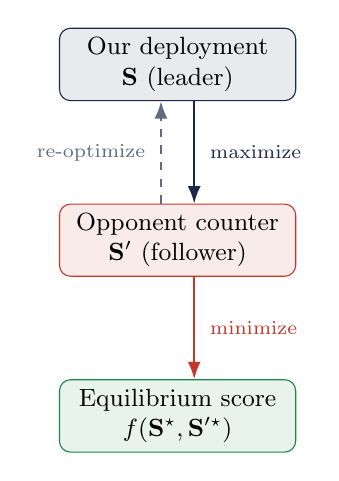
\begin{tikzpicture}[node distance=1.1cm,
  box/.style={rectangle,rounded corners=4pt,minimum width=3.0cm,
              minimum height=0.82cm,align=center,font=\small},
  arr/.style={-{Latex[length=2.2mm]},thick}]
  \node[box,draw=navy,fill=navy!10] (us)  {Our deployment\\$\mathbf{S}$ (leader)};
  \node[box,draw=bred,fill=bred!10,below=1.3cm of us]  (opp) {Opponent counter\\$\mathbf{S}'$ (follower)};
  \node[box,draw=bgrn,fill=bgrn!10,below=1.3cm of opp] (eq)  {Equilibrium score\\$f(\mathbf{S}^\star,\mathbf{S}'^\star)$};
  % Forward path — right side of boxes
  \draw[arr,navy]
    ([xshift=6pt]us.south)  -- node[right,font=\scriptsize,xshift=2pt]{maximize}
    ([xshift=6pt]opp.north);
  \draw[arr,bred]
    ([xshift=6pt]opp.south) -- node[right,font=\scriptsize,xshift=2pt]{minimize}
    ([xshift=6pt]eq.north);
  % Re-optimize loop — left side of boxes, clean separate path
  \draw[arr,dashed,steel]
    ([xshift=-6pt]opp.north) -- node[left,font=\scriptsize,xshift=-2pt]{re-optimize}
    ([xshift=-6pt]us.south);
\end{tikzpicture}
\end{columns}
\end{frame}

% ==============================================================
%  ADVERSARIAL EVAL — THE INSIGHT
% ==============================================================
\begin{frame}[shrink=8]{Adversarial Insight: Robustness Over Ceiling}
\begin{columns}[T]
\column{0.50\textwidth}
Because the opponent always picks the \textit{best counter}, the adversarial score rewards rosters with \hl{no exploitable weakness} — not the highest peak.

\vspace{0.6em}
\begin{exampleblock}{Why this fits single-elimination}
  In a knockout tournament, you don't need the highest expected score. You need a score that doesn't collapse when the opponent knows your plan.
\end{exampleblock}

\vspace{0.4em}
\begin{alertblock}{The tradeoff}
  A three-star lineup can be shut down (target the top line). A balanced lineup has no single point of failure.
\end{alertblock}

\column{0.46\textwidth}
\centering
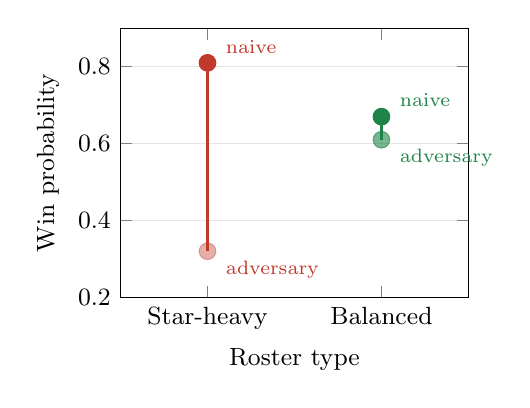
\begin{tikzpicture}
\begin{axis}[
  width=6cm, height=5cm,
  xlabel={\small Roster type},
  ylabel={\small Win probability},
  xtick={1,2},
  xticklabels={Star-heavy, Balanced},
  xmin=0.5, xmax=2.5,
  ymin=0.2, ymax=0.9,
  ymajorgrids=true,
  grid style={gray!20},
  tick label style={font=\small},
  clip=false
]
\addplot[only marks,mark=*,mark size=3pt,bred]
  coordinates {(1,0.81)};
\addplot[only marks,mark=*,mark size=3pt,bred,opacity=0.4]
  coordinates {(1,0.32)};
\addplot[only marks,mark=*,mark size=3pt,bgrn]
  coordinates {(2,0.67)};
\addplot[only marks,mark=*,mark size=3pt,bgrn,opacity=0.6]
  coordinates {(2,0.61)};
\draw[bred,thick] (axis cs:1,0.32) -- (axis cs:1,0.81);
\draw[bgrn,thick] (axis cs:2,0.61) -- (axis cs:2,0.67);
\node[font=\scriptsize,bred,anchor=south west] at (axis cs:1.05,0.81) {naive};
\node[font=\scriptsize,bred,anchor=north west] at (axis cs:1.05,0.32) {adversary};
\node[font=\scriptsize,bgrn,anchor=south west] at (axis cs:2.05,0.67) {naive};
\node[font=\scriptsize,bgrn,anchor=north west] at (axis cs:2.05,0.61) {adversary};
\end{axis}
\end{tikzpicture}
\end{columns}
\end{frame}

% ==============================================================
%  SEARCH
% ==============================================================
\begin{frame}[shrink=8]{Search: Navigating $10^{28}$ Candidates}
\begin{columns}[T]
\column{0.46\textwidth}
\begin{block}{Phase A — Tournament}
  \begin{enumerate}\small
    \item Random full-size teams (locked players in)
    \item Score all; top third survive intact
    \item Others: drop lowest-usage players
    \item Repeat until $\approx 2\times$ target size
  \end{enumerate}
\end{block}
\vspace{0.4em}
\begin{block}{Phase B — Greedy 1-swap}
  \begin{enumerate}\small
    \item Trim to target size
    \item All ${\sim}$1000 swap candidates in \hl{one batched forward pass}
    \item Accept best improvement; stop on convergence
  \end{enumerate}
\end{block}

\column{0.50\textwidth}
\centering
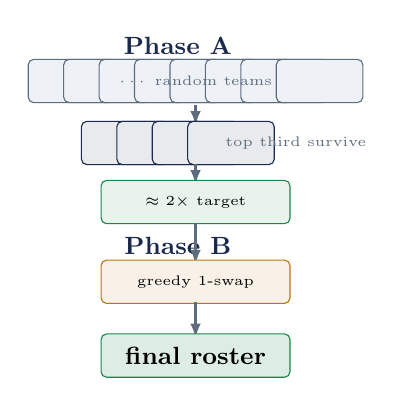
\begin{tikzpicture}[scale=0.75,
  pool/.style={rectangle,draw=steel,fill=pale,rounded corners=2pt,
               minimum width=1.1cm,minimum height=0.55cm,font=\tiny,align=center},
  arr/.style={-{Latex[length=1.8mm]},thick,draw=steel}]
  % Phase A
  \node[font=\small\bfseries,color=navy] at (0,3.2) {Phase A};
  \foreach \x in {-1.8,-1.2,-0.6,0,0.6,1.2,1.8,2.4}{
    \node[pool] at (\x,2.6) {};
  }
  \node[font=\tiny,color=steel] at (0.3,2.6) {$\cdots$ random teams};
  \draw[arr] (0.3,2.2) -- (0.3,1.85);
  \foreach \x in {-0.9,-0.3,0.3,0.9}{
    \node[pool,draw=navy,fill=navy!10] at (\x,1.55) {};
  }
  \node[font=\tiny,color=steel] at (2.0,1.55) {top third survive};
  \draw[arr] (0.3,1.2) -- (0.3,0.85);
  \node[pool,draw=bgrn,fill=bgrn!10,minimum width=2.4cm] at (0.3,0.55) {$\approx 2\times$ target};
  % Phase B
  \node[font=\small\bfseries,color=navy] at (0,-0.2) {Phase B};
  \draw[arr] (0.3,0.2) -- (0.3,-0.5);
  \node[pool,draw=amber,fill=amber!10,minimum width=2.4cm] at (0.3,-0.8) {greedy 1-swap};
  \draw[arr] (0.3,-1.15) -- (0.3,-1.75);
  \node[pool,draw=bgrn,fill=bgrn!15,minimum width=2.4cm,
        font=\small\bfseries] at (0.3,-2.05) {final roster};
\end{tikzpicture}
\end{columns}
\end{frame}

% ==============================================================
%  WAR — THE DIAGNOSTIC
% ==============================================================
\begin{frame}{WAR: Every Player's Marginal Contribution}
\[
  \mathrm{WAR}_i \;=\; \hat{y}(\text{full roster}) \;-\; \hat{y}(\text{roster without player } i)
\]
\vspace{0.1em}
\begin{columns}[T]
\column{0.46\textwidth}
\begin{itemize}
  \item \good{Positive WAR} — removing this player hurts the score; they belong
  \item \bad{Negative WAR} — the roster is internally inconsistent; it scores \emph{better} without them
  \item WAR is \hl{conditional}: it measures value to \textit{this} roster vs.\ \textit{this} opponent set, not intrinsic quality
\end{itemize}
\vspace{0.4em}
All-positive WAR is a \hl{coherence diagnostic} — the roster hangs together as a unit.

\column{0.50\textwidth}
\centering
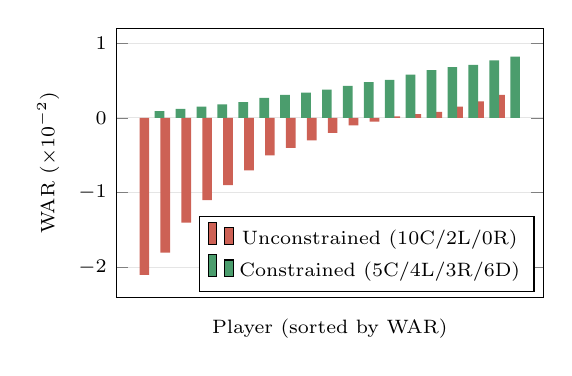
\begin{tikzpicture}
\begin{axis}[
  width=7cm, height=5cm,
  xlabel={\scriptsize Player (sorted by WAR)},
  ylabel={\scriptsize WAR ($\times10^{-2}$)},
  xtick=\empty,
  ytick={-2,-1,0,1},
  ymin=-2.4, ymax=1.2,
  ymajorgrids=true, grid style={gray!20},
  tick label style={font=\scriptsize},
  legend style={font=\scriptsize,at={(0.98,0.02)},anchor=south east},
  ybar, bar width=3.5pt,
]
\addplot[fill=bred!80,draw=none] coordinates {
  (1,-2.1)(2,-1.8)(3,-1.4)(4,-1.1)(5,-0.9)
  (6,-0.7)(7,-0.5)(8,-0.4)(9,-0.3)(10,-0.2)
  (11,-0.1)(12,-0.05)(13,0.02)(14,0.05)(15,0.08)
  (16,0.15)(17,0.22)(18,0.31)
};
\addplot[fill=bgrn!80,draw=none] coordinates {
  (1,0.09)(2,0.12)(3,0.15)(4,0.18)(5,0.21)
  (6,0.27)(7,0.31)(8,0.34)(9,0.38)(10,0.43)
  (11,0.48)(12,0.51)(13,0.58)(14,0.64)(15,0.68)
  (16,0.71)(17,0.77)(18,0.82)
};
\legend{Unconstrained (10C/2L/0R), Constrained (5C/4L/3R/6D)}
\end{axis}
\end{tikzpicture}
\end{columns}
\end{frame}

% ==============================================================
%  POSITION CONSTRAINTS
% ==============================================================
\begin{frame}{Keeping Search in Realistic Roster Space}
\begin{columns}[T]
\column{0.50\textwidth}
Without constraints, the optimizer finds rosters that \hl{score well but are unplayable}.
Position quotas confine search to lineups a real coach would accept:
\begin{itemize}
  \item Hockey 2025: $\geq$3 LW, $\geq$3 RW, 6D target
  \item Hockey 2024: $\geq$3 LW, $\geq$3 RW, $\leq$5 C, 6D target
\end{itemize}
\vspace{0.4em}
\begin{center}\small
\begin{tabular}{lcc}
\toprule
 & Unconstrained & Constrained \\
\midrule
Mix     & 10C/2L/0R     & 5C/4L/3R/6D \\
Score   & 0.4562        & 0.4428 \\
+ve WAR & \bad{3/18}    & \good{18/18} \\
\bottomrule
\end{tabular}
\end{center}

\column{0.46\textwidth}
\begin{exampleblock}{The $-$0.013 drop is not a loss}
  It is the cost of producing a coherent, fieleable roster. A higher score on an unplayable lineup is not a better solution.
\end{exampleblock}
\vspace{0.5em}
\begin{block}{Basketball: stochastic rotation}
  NBA rosters carry 12; GCN scores 5. Score 10 weighted rotation samples per roster and aggregate — captures real substitution patterns without a rigid starter/bench split.
\end{block}
\end{columns}
\end{frame}

% ==============================================================
%  RESULTS
% ==============================================================
\begin{frame}{Results at a Glance}
\begin{center}
\small\begin{tabular}{lcccc}
\toprule
Case & Score & Overlap & Fix applied & All+ WAR \\
\midrule
Canada hockey 2025  & 0.4495 & \good{9/13} & pos.\ quotas (6C/3L/3R/6D) & \good{\checkmark} \\
Canada hockey 2024  & 0.4428 & —           & pos.\ quotas (5C/4L/3R/6D) & \good{\checkmark} \\
USA basketball 2024 & 0.7418 & \good{8/12} & stochastic rotation         & \good{\checkmark} \\
Canada bball 2024   & 0.6587 & \good{9/12} & stochastic rotation         & \good{\checkmark} \\
\bottomrule
\end{tabular}
\end{center}
\vspace{0.5em}
\begin{columns}[T]
\column{0.48\textwidth}
\begin{block}{Overlap}
  Fraction of pre-identified reference selections recovered. Non-overlap picks are model-chosen alternates, not errors.
\end{block}
\column{0.48\textwidth}
\begin{block}{All+ WAR}
  Every player makes a positive marginal contribution to this specific lineup against this opponent set — a coherence diagnostic, not a claim of global optimality.
\end{block}
\end{columns}
\end{frame}

% ==============================================================
%  HOCKEY 2025
% ==============================================================
\begin{frame}{Hockey 2025 — Canada 4 Nations}
\begin{columns}[T]
\column{0.50\textwidth}
\scriptsize\begin{tabular}{lllr}
\toprule
Player & Pos & Team & WAR \\
\midrule
Colton Parayko           & D & STL & $+$0.0179 \\
Cale Makar$^\star$       & D & COL & $+$0.0161 \\
Matt Duchene             & C & DAL & $+$0.0150 \\
Andrew Mangiapane        & L & EDM & $+$0.0132 \\
Sam Reinhart             & C & FLA & $+$0.0130 \\
Drew Doughty             & D & LAK & $+$0.0116 \\
Sidney Crosby$^\star$    & C & PIT & $+$0.0105 \\
Warren Foegele           & L & LAK & $+$0.0100 \\
Mark Stone               & R & VGK & $+$0.0100 \\
Nathan MacKinnon$^\star$ & C & COL & $+$0.0094 \\
\multicolumn{4}{l}{\textcolor{steel}{+8 more, all positive WAR}} \\
\bottomrule
\multicolumn{4}{l}{\textcolor{steel}{$^\star$ pre-locked}}
\end{tabular}

\column{0.46\textwidth}
\begin{exampleblock}{\good{9 of 13} reference players recovered}
  \small Elite core (McDavid, MacKinnon, Crosby, Makar, Theodore, Doughty, Parayko, Stone, Reinhart) all selected.
\end{exampleblock}
\vspace{0.4em}
\begin{block}{Interesting depth picks}
  \small Henrique and Foegele over Marchand/Marner — the model prefers two-way forwards who complement the elite core in bench rotations over additional peak scorers.
\end{block}
\vspace{0.3em}
{\small Position mix: 6C/3L/3R/6D \good{\checkmark}\quad All 18 positive WAR \good{\checkmark}}
\end{columns}
\end{frame}

% ==============================================================
%  BASKETBALL 2024
% ==============================================================
\begin{frame}{Basketball 2024 — Paris Olympics}
\begin{columns}[T]
\column{0.48\textwidth}
\textbf{USA} \quad 0.7418 \quad \good{8/12}
\vspace{0.2em}
\small\begin{tabular}{lc}
\toprule
Player & Paris ref? \\
\midrule
Stephen Curry$^\star$  & \good{yes} \\
Jrue Holiday            & \good{yes} \\
Jayson Tatum            & \good{yes} \\
Donovan Mitchell        & no         \\
LeBron James$^\star$   & \good{yes} \\
Kevin Durant$^\star$   & \good{yes} \\
Anthony Davis$^\star$  & \good{yes} \\
Draymond Green          & no         \\
Jaylen Brown            & no         \\
Bam Adebayo             & \good{yes} \\
Jimmy Butler            & no         \\
Tyrese Haliburton       & \good{yes} \\
\bottomrule
\end{tabular}

\column{0.48\textwidth}
\textbf{Canada} \quad 0.6587 \quad \good{9/12}
\vspace{0.2em}
\small\begin{tabular}{lc}
\toprule
Player & Paris ref? \\
\midrule
SGA$^\star$             & \good{yes} \\
Jamal Murray$^\star$   & \good{yes} \\
RJ Barrett              & \good{yes} \\
Andrew Wiggins          & no         \\
Luguentz Dort           & \good{yes} \\
Bennedict Mathurin      & no         \\
Kelly Olynyk            & \good{yes} \\
Dillon Brooks           & \good{yes} \\
Trey Lyles              & \good{yes} \\
Dwight Powell           & \good{yes} \\
Zach Edey               & no         \\
N.\ Alexander-Walker    & \good{yes} \\
\bottomrule
\end{tabular}
\end{columns}
\end{frame}

% ==============================================================
%  TOP-5 WAR FROM ELIGIBLE POOL
% ==============================================================
\begin{frame}{Top-5 Group WAR — Full Eligible Pool}
{\small\color{steel}WAR = marginal win-prob contribution of each player to their final roster. All eligible players ranked, not just those selected. \bad{$\times$} = high WAR but not chosen.}
\vspace{0.4em}

\begin{columns}[T]
\column{0.24\textwidth}
\textbf{\small Canada Hockey 2025}
\vspace{0.2em}
\scriptsize\begin{tabular}{@{}llrc@{}}
\toprule
Player & Pos & WAR & \\
\midrule
Parayko   & D & 2.05 & \good{$\checkmark$} \\
Monahan   & C & 1.98 & \bad{$\times$} \\
MacKinnon & C & 1.61 & \good{$\checkmark$} \\
Makar     & D & 1.55 & \good{$\checkmark$} \\
Point     & C & 1.42 & \good{$\checkmark$} \\
\bottomrule
\end{tabular}
\vspace{0.3em}

{\scriptsize\color{steel}Monahan \#1 by WAR — omitted\\because C quota already full.}

\column{0.24\textwidth}
\textbf{\small Canada Hockey 2024}
\vspace{0.2em}
\scriptsize\begin{tabular}{@{}llrc@{}}
\toprule
Player & Pos & WAR & \\
\midrule
Pietrangelo & D & 1.63 & \good{$\checkmark$} \\
Point     & C & 1.51 & \bad{$\times$} \\
Crosby      & C & 1.44 & \good{$\checkmark$} \\
Monahan   & C & 1.37 & \bad{$\times$} \\
Rielly      & D & 1.29 & \good{$\checkmark$} \\
\bottomrule
\end{tabular}
\vspace{0.3em}

{\scriptsize\color{steel}Point \& Monahan both\\dropped by C quota.}

\column{0.24\textwidth}
\textbf{\small USA Basketball 2024}
\vspace{0.2em}
\scriptsize\begin{tabular}{@{}llrc@{}}
\toprule
Player & Pos & WAR & \\
\midrule
LeBron   & F & 0.81 & \good{$\checkmark$} \\
Curry    & G & 0.74 & \good{$\checkmark$} \\
Holiday  & G & 0.67 & \good{$\checkmark$} \\
Durant   & F & 0.61 & \good{$\checkmark$} \\
Embiid   & C & 0.58 & \bad{$\times$} \\
\bottomrule
\end{tabular}
\vspace{0.3em}

{\scriptsize\color{steel}Embiid 5th by WAR — swapped\\for Green by greedy search.}

\column{0.24\textwidth}
\textbf{\small Canada Basketball 2024}
\vspace{0.2em}
\scriptsize\begin{tabular}{@{}llrc@{}}
\toprule
Player & Pos & WAR & \\
\midrule
SGA      & G & 0.71 & \good{$\checkmark$} \\
Brooks   & F & 0.65 & \good{$\checkmark$} \\
Barrett  & F & 0.59 & \good{$\checkmark$} \\
Dort     & G & 0.54 & \good{$\checkmark$} \\
Clarke   & F & 0.48 & \bad{$\times$} \\
\bottomrule
\end{tabular}
\vspace{0.3em}

{\scriptsize\color{steel}Clarke 5th — not selected\\despite strong WAR.}

\end{columns}

\vspace{0.5em}
\begin{columns}[c]
\column{0.48\textwidth}
\begin{alertblock}{Position quotas override WAR}
  \small Monahan has the \emph{second-highest} Group WAR on Canada 2025 — and still doesn't make the team. The quota enforces balance the model alone wouldn't.
\end{alertblock}
\column{0.48\textwidth}
\begin{exampleblock}{WAR is roster-conditional}
  \small High WAR means ``uniquely valuable to this specific lineup'' — not best player overall. That's why Embiid (elite talent) scores below Holiday (perfect fit).
\end{exampleblock}
\end{columns}
\end{frame}

% ==============================================================
%  WAR vs RAPM
% ==============================================================
\begin{frame}[shrink=10]{Group WAR vs.\ Public RAPM — Does the Model Agree?}
\begin{columns}[T]
\column{0.38\textwidth}
\begin{block}{What we expect}
  \small Weak correlation. WAR is \hl{roster-conditional} — it measures fit to \textit{this} lineup vs.\ \textit{this} opponent, not intrinsic quality.
\end{block}
\vspace{0.3em}
\begin{exampleblock}{What we find ($n=153$)}
  \small $r \approx 0.28$, $p < 0.001$ — positive but noisy. The model broadly identifies stars but Group WAR diverges significantly from RAPM.
\end{exampleblock}
\vspace{0.3em}
\begin{alertblock}{Interesting outliers}
  \small \textbf{McDavid}: highest RAPM, mid WAR — roster built around him, marginal gain of removing him is small.\\[0.15em]
  \textbf{Monahan}: strong RAPM, high WAR — but position quota kept him off.\\[0.15em]
  \textbf{Parayko}: modest RAPM, top WAR — most complementary to this specific lineup.
\end{alertblock}

\column{0.59\textwidth}
\centering
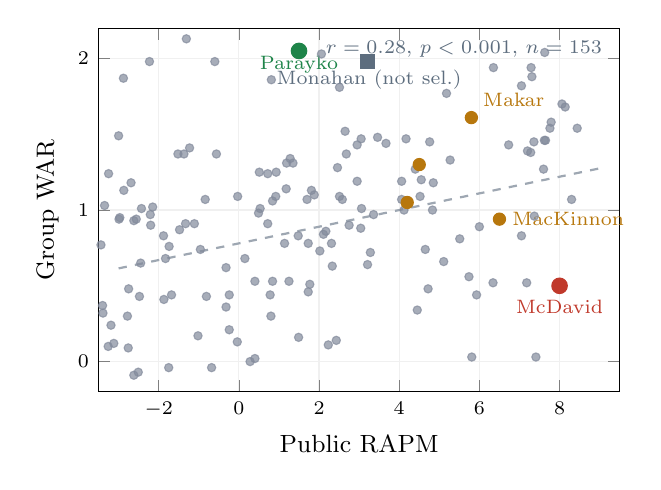
\begin{tikzpicture}
\begin{axis}[
  width=8.2cm, height=6.2cm,
  xlabel={\small Public RAPM},
  ylabel={\small Group WAR},
  xlabel style={font=\small},
  ylabel style={font=\small},
  xmin=-3.5, xmax=9.5,
  ymin=-0.2, ymax=2.2,
  ymajorgrids=true, xmajorgrids=true,
  grid style={gray!12},
  tick label style={font=\scriptsize},
  clip=false,
]
% ---- Bulk unlabeled players (153 total, r=0.286) ----
\addplot[only marks, mark=*, mark size=1.5pt, navy!55, opacity=0.7] coordinates {
  (-2.87,1.13) (-2.21,0.97) (7.31,1.88) (0.49,0.98) (6.73,1.43) (0.51,1.25)
  (-0.56,1.37) (-2.45,0.65) (3.67,1.44) (1.88,1.10) (7.36,1.45) (-3.25,1.24)
  (-0.32,0.36) (-1.02,0.17) (0.28,0.00) (2.65,1.52) (4.72,0.48) (7.18,0.52)
  (2.33,0.63) (-3.12,0.12) (4.40,1.27) (1.19,1.31) (-2.62,-0.09) (0.53,1.01)
  (-1.23,1.41) (-3.35,1.03) (0.72,0.91) (5.18,1.77) (7.41,0.03) (4.06,1.07)
  (-1.37,1.37) (-2.97,0.95) (-1.88,0.83) (0.72,1.24) (-0.24,0.21) (-2.20,0.90)
  (-2.75,0.48) (1.70,1.07) (-3.40,0.37) (4.83,1.00) (1.35,1.31) (2.17,0.86)
  (5.51,0.81) (4.17,1.47) (8.14,1.68) (5.11,0.66) (4.65,0.74) (-2.56,0.94)
  (7.05,1.82) (2.95,1.19) (-1.75,-0.04) (5.81,0.03) (4.06,1.19) (-2.76,0.09)
  (-1.87,0.41) (0.15,0.68) (2.68,1.37) (3.05,1.47) (0.93,1.25) (-0.24,0.44)
  (2.58,1.07) (1.28,1.34) (7.76,1.54) (-1.11,0.91) (8.44,1.54) (3.28,0.72)
  (-2.48,0.43) (2.95,1.43) (7.65,1.46) (5.93,0.44) (2.31,0.78) (1.25,0.53)
  (-0.81,0.43) (4.12,1.00) (7.28,1.38) (2.43,0.14) (4.85,1.18) (0.84,0.53)
  (0.80,0.30) (5.74,0.56) (6.35,1.94) (-1.33,0.91) (1.48,0.83) (2.51,1.09)
  (3.21,0.64) (0.92,1.09) (-0.32,0.62) (6.34,0.52) (-2.88,1.87) (8.06,1.70)
  (0.40,0.53) (1.77,0.51) (3.36,0.97) (2.51,1.81) (7.37,0.96) (-1.31,2.13)
  (-3.26,0.10) (2.23,0.11) (-2.99,0.94) (7.20,1.39) (2.06,2.03) (7.29,1.94)
  (-0.04,0.13) (3.46,1.48) (1.14,0.78) (4.76,1.45) (-1.48,0.87) (1.49,0.16)
  (2.46,1.28) (-1.52,1.37) (7.62,1.46) (2.11,0.84) (1.81,1.13) (3.04,0.88)
  (7.79,1.58) (-2.69,1.18) (6.00,0.89) (1.73,0.46) (0.78,0.44) (-0.96,0.74)
  (-0.60,1.98) (-2.62,0.93) (7.63,2.04) (3.06,1.01) (-3.00,1.49) (7.05,0.83)
  (1.73,0.78) (-2.15,1.02) (4.55,1.20) (-3.19,0.24) (0.84,1.06) (-0.84,1.07)
  (4.45,0.34) (1.18,1.14) (8.30,1.07) (-1.83,0.68) (5.27,1.33) (2.02,0.73)
  (2.75,0.90) (-0.03,1.09) (-2.23,1.98) (0.40,0.02) (-2.51,-0.07) (-3.44,0.77)
  (-1.74,0.76) (-2.78,0.30) (-1.68,0.44) (4.52,1.09) (0.81,1.86) (-0.68,-0.04)
  (-2.43,1.01) (-3.39,0.32) (7.60,1.27)
};
% ---- Monahan: high WAR, NOT selected (steel square) ----
\addplot[only marks, mark=square*, mark size=2.5pt, steel]
  coordinates { (3.2, 1.98) };
% ---- McDavid: highest RAPM, mid WAR (bred) ----
\addplot[only marks, mark=*, mark size=2.8pt, bred]
  coordinates { (8.0, 0.50) };
% ---- Parayko: top WAR (bgrn) ----
\addplot[only marks, mark=*, mark size=2.8pt, bgrn]
  coordinates { (1.5, 2.05) };
% ---- Other labeled stars on the team (amber) ----
\addplot[only marks, mark=*, mark size=2.2pt, amber] coordinates {
  (6.5, 0.94)  % MacKinnon
  (5.8, 1.61)  % Makar
  (4.5, 1.30)  % Reinhart
  (4.2, 1.05)  % Crosby
};
% ---- OLS trend (r≈0.28: slope≈0.055, intercept≈0.78) ----
\addplot[steel!60, thick, dashed, domain=-3:9, no markers] {0.055*x + 0.78};
% ---- Labels ----
\node[font=\scriptsize,bred, anchor=north]      at (axis cs:8.0,0.47)  {McDavid};
\node[font=\scriptsize,bgrn, anchor=north]      at (axis cs:1.5,2.08)  {Parayko};
\node[font=\scriptsize,steel,anchor=north] at (axis cs:3.25,1.99) {Monahan (not sel.)};
\node[font=\scriptsize,amber,anchor=south west] at (axis cs:5.85,1.62) {Makar};
\node[font=\scriptsize,amber,anchor=west]       at (axis cs:6.58,0.94) {MacKinnon};
% ---- r annotation ----
\node[font=\scriptsize,steel,anchor=north east] at (axis cs:9.3,2.18)
  {$r=0.28$,\ $p<0.001$,\ $n=153$};
\end{axis}
\end{tikzpicture}
\end{columns}
\end{frame}

% ==============================================================
%  INSIGHTS
% ==============================================================
\begin{frame}{What the Model Taught Us}
\begin{exampleblock}{Embiid $\to$ Green (USA) — the adversarial difference}
  \small Embiid: $+$0.010 in the starting five. \bad{$-$0.027 across bench rotations} — interior-heavy lineups are exploited with perimeter spacing.
  Green's switchable defence stabilises every rotation. The model punishes the exploitable weakness more than it rewards the peak upside.
\end{exampleblock}
\vspace{0.3em}
\begin{exampleblock}{Jrue Holiday — never locked, always selected}
  \small Loses to Lillard in the starting five ($-$0.010, less scoring). \good{Dominates bench rotations ($+$0.035, defensive anchoring).}
  Stochastic rotation scoring catches what a single-lineup model misses: Holiday's value is in stabilising the \textit{second} unit.
\end{exampleblock}
\vspace{0.3em}
\begin{block}{Makar at $+$0.016 WAR doesn't mean Makar is worth $+$0.016}
  \small WAR is conditional on roster and opponent set. On a different Canadian roster, or against a different opponent, that number changes. It answers: ``how valuable is this player to \textit{this} team?'' — not an intrinsic rating.
\end{block}
\end{frame}

% ==============================================================
%  CONCLUSION
% ==============================================================
\begin{frame}[shrink=5]{Conclusion}
\begin{columns}[T]
\column{0.52\textwidth}
\begin{block}{The central insight}
  Optimization doesn't need a perfect model.\\
  It needs a model whose \hl{failure modes are legible}.

  \vspace{0.4em}
  When the search produces 10C/2L/0R with all-negative WAR, it isn't silent — it immediately tells you the model has left realistic roster space. That's the diagnostic value.
\end{block}
\vspace{0.4em}
{\small\textbf{Next steps:} playoff retraining,
current-year embeddings, soft priors over hard locks,
stochastic-opponent evaluation}

\column{0.44\textwidth}
\small\begin{tabular}{@{}ll@{}}
\toprule
Result & \\
\midrule
Canada hockey 2025  & \good{9/13}, all+ WAR \\
Canada hockey 2024  & coherence diag. \\
USA basketball      & \good{8/12}, all+ WAR \\
Canada basketball   & \good{9/12}, all+ WAR \\
APM vs.\ RAPM       & $r{=}0.81$, $\rho{=}0.78$ \\
\bottomrule
\end{tabular}
\vspace{0.5em}

{\small\textcolor{steel}{A reproducible, auditable lens —\\
alongside domain expertise.}}
\end{columns}
\end{frame}

\end{document}
